\documentclass[12pt, a4paper]{article}
\usepackage[utf8]{inputenc}
\usepackage[russian]{babel}
\usepackage{amsmath}
\usepackage{amsfonts}
\usepackage{amssymb}
\usepackage{graphicx}
\usepackage{geometry}
\usepackage{caption}
\usepackage{subcaption}
\usepackage{float}
\usepackage[labelformat=empty]{subcaption}  % в преамбуле

\geometry{left=1.5cm, right=1.5cm, top=1.5cm, bottom=1.5cm}



\begin{document}

\title{\begin{center}Лабораторная работа №4.7.2:\end{center}
Эффект Поккельса}
\author{Струков О. И. \\ Б04-404}
\date{}

\thispagestyle{empty}
\pagenumbering{gobble}
\maketitle
\newpage
\pagenumbering{arabic}

\section*{Теоретическая часть}

\subsection*{Эффект Поккельса}

Эффектом Поккельса называется изменение показателя преломления света в кристалле под действием электрического поля, причём это изменение пропорционально напряжённости электрического поля. Вследствие эффекта Поккельса в кристалле либо появляется двойное лучепреломление, либо меняется его величина (если кристалл был двулучепреломляющим в отсутствие поля), либо, как в данной работе, одноосный кристалл становится двуосным.

Изменение показателя преломления кристаллов под действием внешнего электрического поля происходит за счёт анизотропных свойств кристаллов. Под действием постоянного электрического поля электроны смещаются в сторону того или иного иона (в случае кристалла ниобата лития LiNbO$_3$ --- это ион Li или Nb), при этом меняется поляризуемость среды и связанный с ней показатель преломления.

\subsection*{Интерференционная картина}

Если перед кристаллом, помещённым между скрещенными поляроидами, расположить линзу или матовую пластинку, после которых лучи будут рассеиваться под различными углами, то на экране, расположенном за поляроидом, можно увидеть тёмные концентрические окружности (коноскопическую картину) --- результат интерференции обыкновенной и необыкновенной волн.

Разность фаз между обыкновенной и необыкновенной волнами, приобретаемая при прохождении через кристалл длиной $\ell$, равна:
\begin{equation}
\Delta\varphi = \frac{2\pi}{\lambda} \cdot \ell \cdot (n_1 - n_2)
\end{equation}

Для малых углов получаем:
\begin{equation}
n_2 \approx n_o - (n_o - n_e)\theta^2
\end{equation}

Таким образом:
\begin{equation}
\Delta\varphi = \frac{2\pi}{\lambda}\ell(n_o - n_e)\theta^2
\end{equation}

Для $m$-го тёмного кольца $\Delta\varphi = 2\pi m$, откуда выражение для радиуса кольца:
\begin{equation}
r_m^2 = \frac{\lambda}{\ell}\frac{(n_o L)^2}{(n_o - n_e)}m
\end{equation}

\subsection*{Электрооптический эффект}

При наложении электрического поля $E_{\text{эл}}$, направленного вдоль оси $x$, перпендикулярной оптической оси кристалла $z$, в плоскости $(xy)$ возникают два главных направления $\xi$ и $\eta$ под углами $45^\circ$ к осям $x$ и $y$ с показателями преломления $(n_o - \Delta n)$ и $(n_o + \Delta n)$, где $\Delta n = A \cdot E_{\text{эл}}$ ($A$ --- константа, зависящая от типа кристалла).

Разность фаз:
\begin{equation}
\Delta\varphi = \frac{2\pi\ell}{\lambda} 2\Delta n = \frac{4\pi\ell}{\lambda} A E_{\text{эл}} = \frac{4\pi}{\lambda}\frac{\ell}{d} A U
\end{equation}

где $U = E_{\text{эл}} d$ --- напряжение на кристалле, $d$ --- размер кристалла в поперечном направлении.

Интенсивность света на выходе:
\begin{equation}
I_{\text{вых}} = I_0 \sin^2\left(\frac{\Delta\varphi}{2}\right) = I_0 \sin^2\left(\frac{\pi}{2}\frac{U}{U_{\lambda/2}}\right)
\end{equation}

Полуволновое напряжение:
\begin{equation}
U_{\lambda/2} = \frac{\lambda d}{4A\ell}
\end{equation}

\begin{figure}[H]
\centering
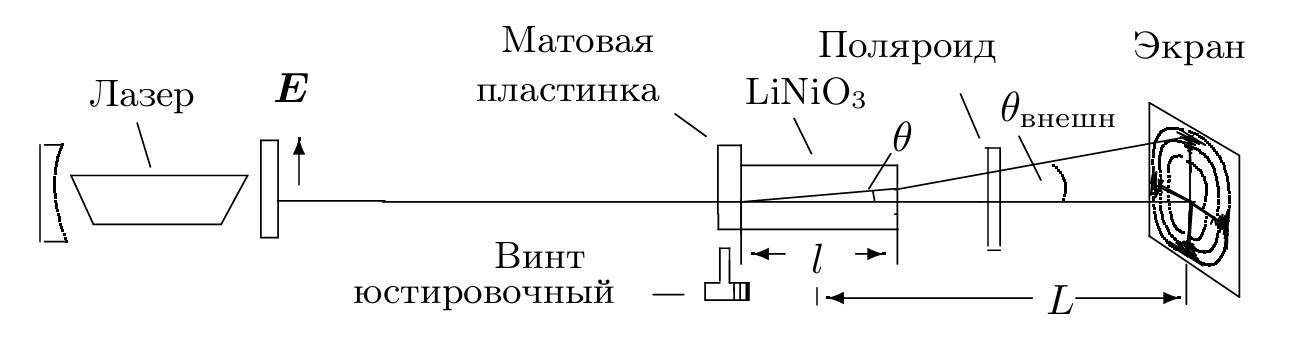
\includegraphics[width=0.8\textwidth]{fig1.jpg}
\caption{Схема для наблюдения интерференционной картины}
\label{fig:scheme1}
\end{figure}

\begin{figure}[H]
\centering
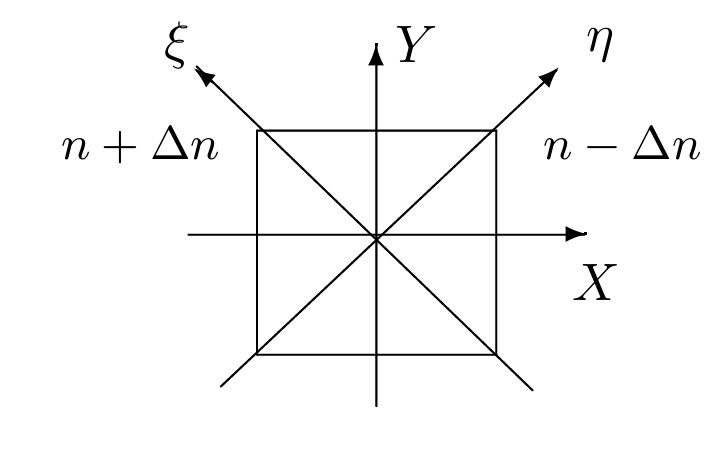
\includegraphics[width=0.5\textwidth]{fig2.jpg}
\caption{Эффект Поккельса -- появление новых главных направлений при наложении электрического поля}
\label{fig:pockels}
\end{figure}

\begin{figure}[H]
\centering
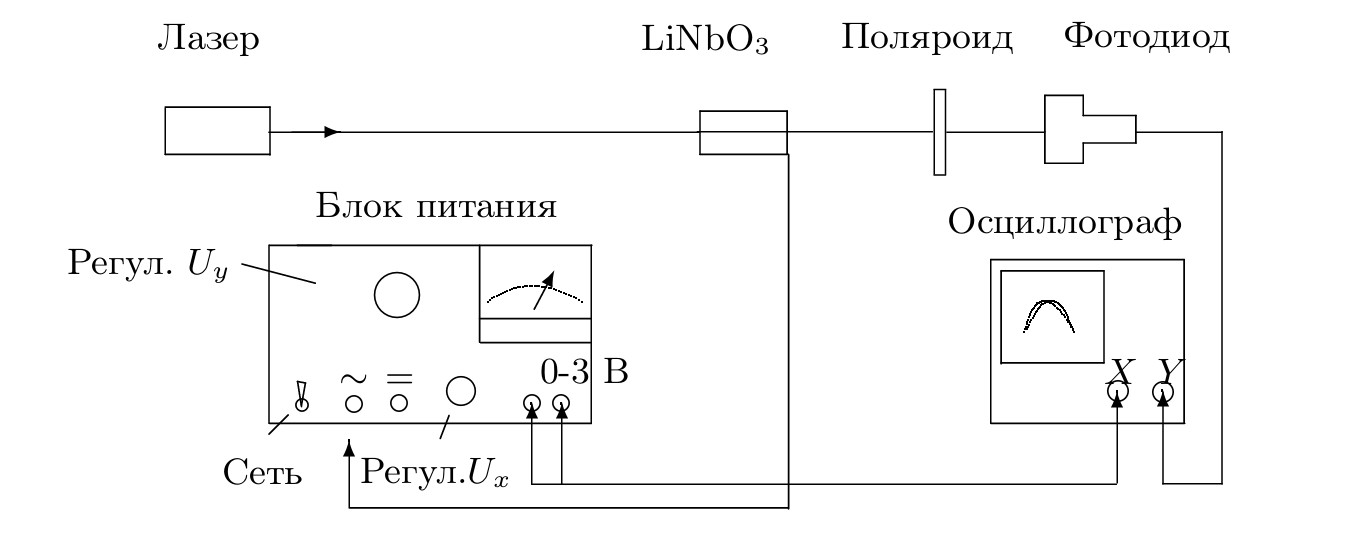
\includegraphics[width=0.8\textwidth]{fig3.jpg}
\caption{Схема для изучения двойного лучепреломления в электрическом поле}
\label{fig:scheme2}
\end{figure}

\section*{Ход работы}

% \subsection*{Юстировка системы}
% Для проверки вертикальной поляризации лазерного луча было определено разрешённое направление анализатора: через поляроид был рассмотрен дневной свет от окна, отражённый от светлой поверхности (стола, подоконника); вращая поляроид, был найден минимум освещённости и замечен отсчёт угла на лимбе. Вблизи угла Брюстера в отражённом свете преобладает компонента светового вектора, параллельная плоскости стола («правило иголки»), следовательно, минимум отражённого света соответствует вертикальному разрешённому направлению поляроида.
    
\begin{enumerate}
    \item Была собрана оптическая схема согласно рис. \ref{fig:scheme1}, поставлен кристалл и установлена перед ним вплотную к кювете матовая пластинка. Расстояние от кристалла до экрана было установлено в пределах 70--80 см. %(оптимальное расстояние для тёмной комнаты, в светлое время дня --- около 30 см).
    
    \item На экране была получена интерференционная картина, её фотография приведена на рис. 4:%. Отклоняя кристалл с помощью юстировочного винта и поворачивая рейтер с кюветой вокруг вертикальной оси, было достигнуто совмещение центра коноскопической картины с положением луча на экране в отсутствие матовой пластинки.
    
    % Анализатор был повёрнут на $90^\circ$, и было убеждено, что коноскопическая картина изменилась на негативную. Анализатор был возвращён в прежнее положение (горизонтальное разрешённое направление).
% \end{enumerate}

\begin{figure}[H]
\centering

\includegraphics[width=0.6\textwidth]{1.jpg}
\caption{Фотография интерференционной картины}
\label{fig:interference}
\end{figure}

% \subsection*{Измерения}

% \begin{enumerate}
    % \setcounter{enumi}{3}
    \item Были измерены радиусы интерференционных колец $r(m)$ и расстояние $L= (76\pm0,5)$ см от середины кристалла до экрана. Длина волны лазера $\lambda = 0,63$ мкм, показатель преломления для обыкновенной волны $n_0 = 2,29$, длина кристалла $\ell = 26$ мм.
    
    % \textbf{Измеренные данные:}
    % \begin{itemize}
    %     \item Расстояние от кристалла до экрана: $L = (76\pm0,5)$ см
    %     \item Длина кристалла: $\ell = \ldots$ см
    %     \item Длина волны лазера: $\lambda = 0.63$ мкм
    %     \item Показатель преломления: $n_o = 2.29$
    % \end{itemize}
    
    % \begin{table}[h]
    % \centering
    % \caption{Измерение радиусов интерференционных колец}
    % \begin{tabular}{|c|c|c|}
    % \hline
    % $m$ & $r$, мм & $r^2$, мм$^2$ \\
    % \hline
    % 1 & & \\
    % 2 & & \\
    % 3 & & \\
    % 4 & & \\
    % 5 & & \\
    % \hline
    % \end{tabular}
    % \end{table}
    
\begin{table}[H]
\centering
\begin{tabular}{|c|c|c|}
\hline
$m$ & $r$, мм & $r^2$, мм$^2$ \\
\hline
1 & $32,0 \pm 0,5$ & $1024,00 \pm 32,0$ \\ \hline
2 & $42,5 \pm 0,5$ & $1806,25 \pm 42,5$ \\ \hline
3 & $50,5 \pm 0,5$ & $2550,25 \pm 50,5$ \\ \hline
4 & $57,0 \pm 0,5$ & $3249,00 \pm 57,0$ \\ \hline
5 & $63,3 \pm 0,5$ & $4000,56 \pm 63,3$ \\ \hline
6 & $68,5 \pm 0,5$ & $4692,25 \pm 68,5$ \\ \hline
7 & $73,5 \pm 0,5$ & $5402,25 \pm 73,5$ \\ \hline
8 & $78,8 \pm 0,5$ & $6201,56 \pm 78,8$ \\
\hline
\end{tabular}
\caption{Радиусы интерференционных колец}
\end{table}


    Был построен график $r^2 = f(m)$ (рис. 5). Из формулы $r_m^2 = \dfrac{\lambda}{\ell}\dfrac{(n_o L)^2}{(n_o - n_e)}m = k m$ по углу наклона прямой $k = (734,10 \pm 8,28)$ мм$^2$ было определено двулучепреломление $(n_o - n_e)$ ниобата лития: $(n_o - n_e) = \dfrac{\lambda}{\ell}\dfrac{(n_o L)^2}{k} = 0,09998 \pm 0,00173$
    
    \begin{figure}[H]
    \centering
    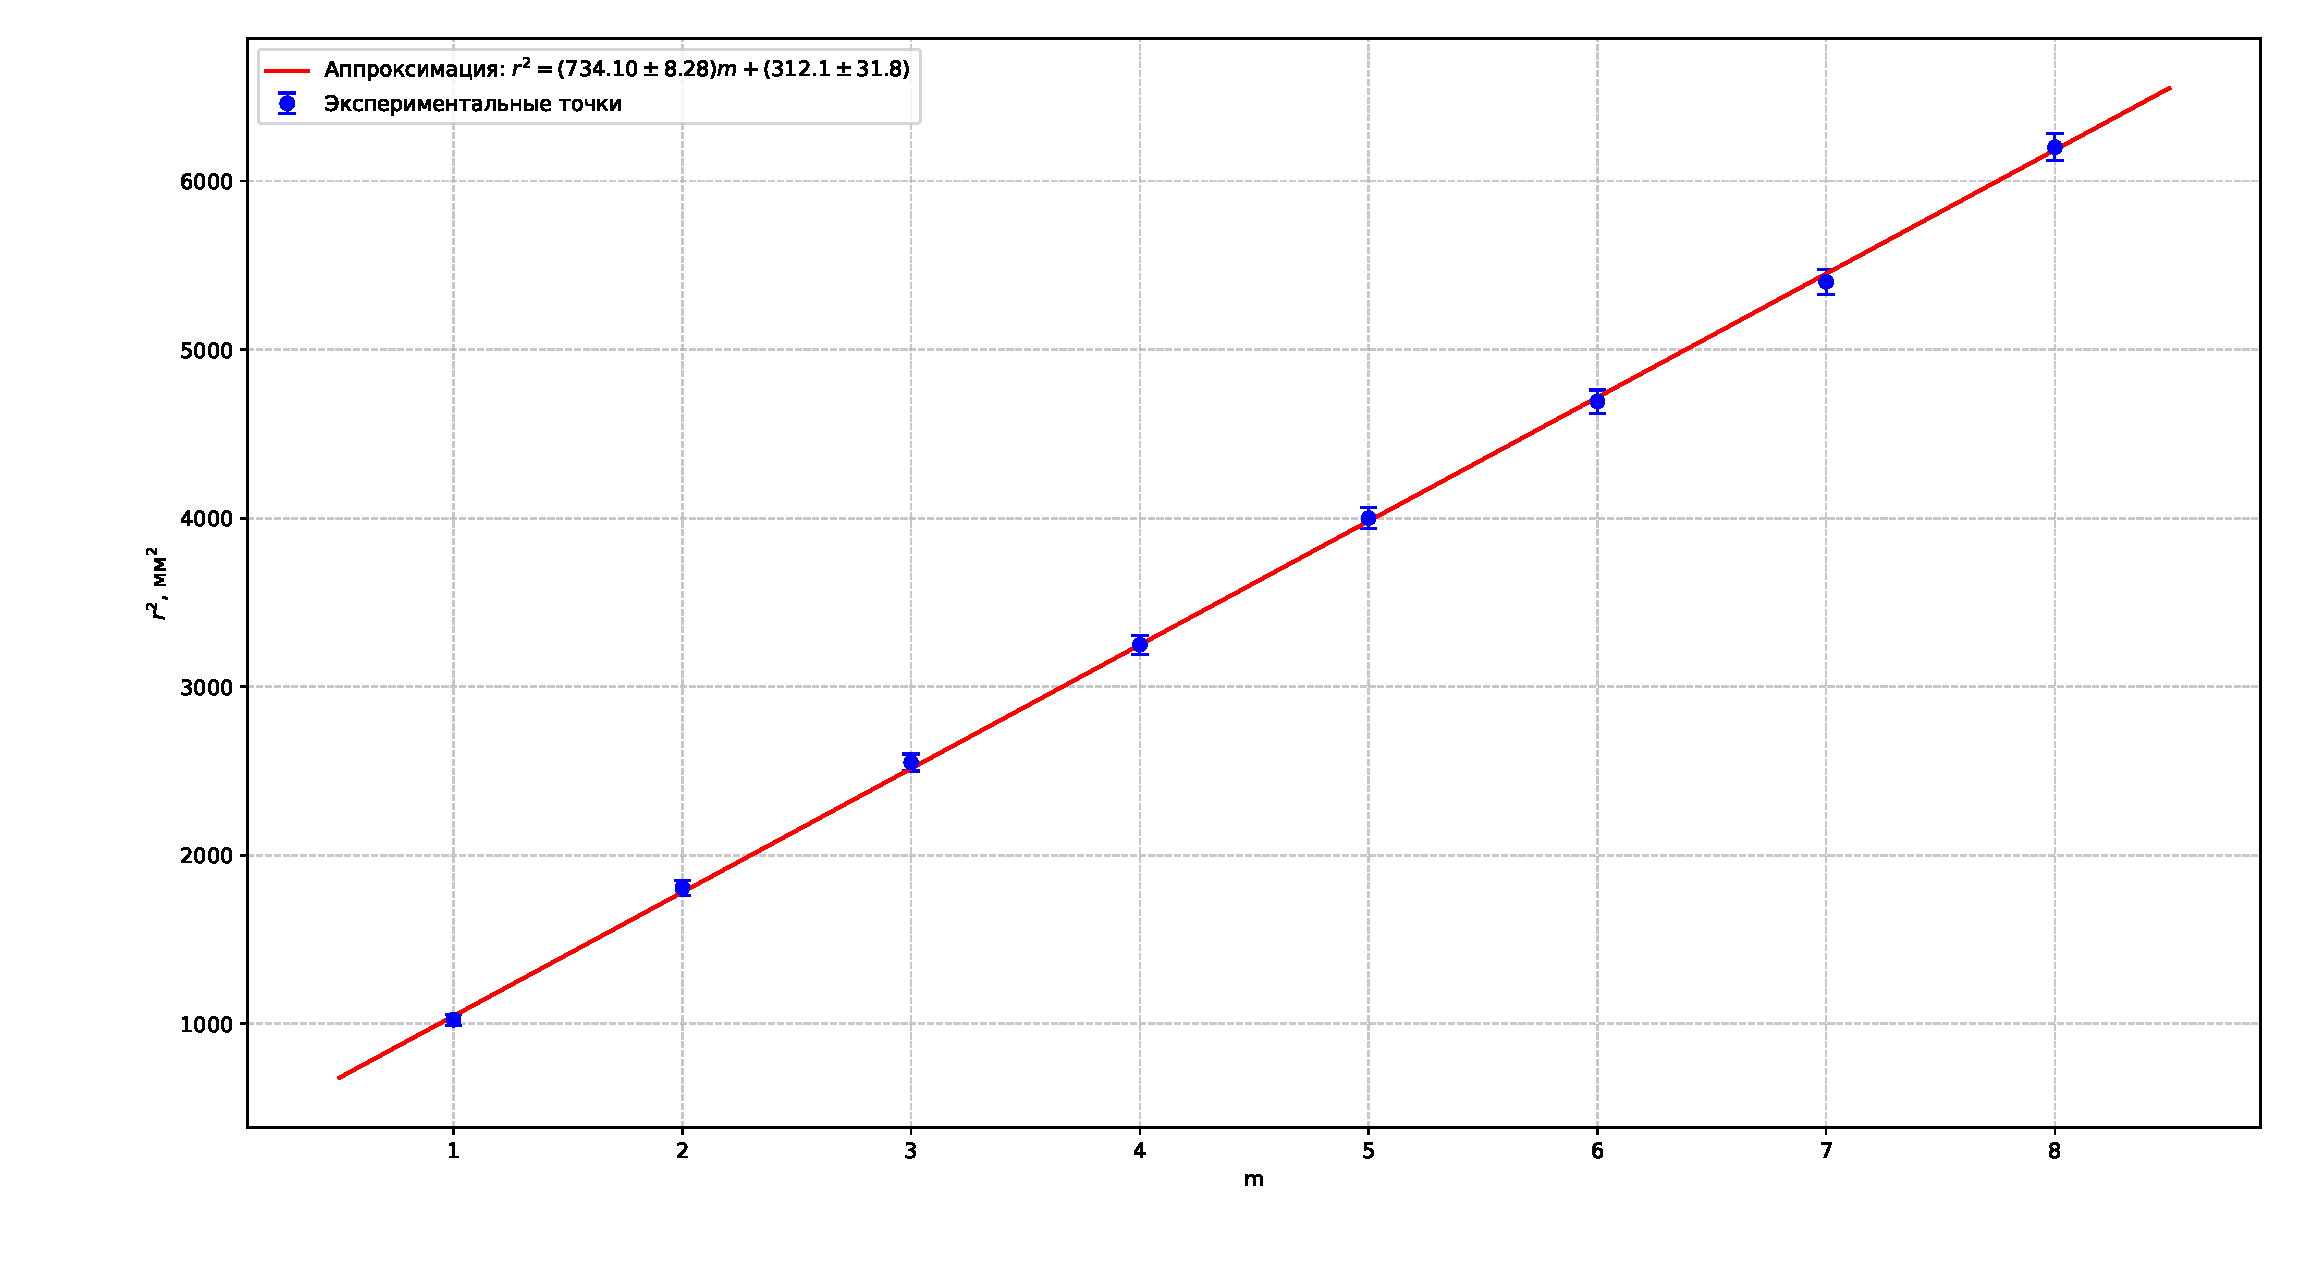
\includegraphics[width=0.8\textwidth]{r2m.pdf}
    \caption{График зависимости $r^2$ от $m$}
    \label{fig:graph}
    \end{figure}
    
    \item Была убрана матовая пластинка. Был подключён разъём блока питания на постоянное напряжение, установлен регулятор напряжения на минимальное напряжение и включён блок питания в сеть.
    
    С увеличением напряжения на кристалле яркость пятна на экране увеличивалась и достигала максимума при $U = U_{\lambda/2}$. При $U = 2U_{\lambda/2} = U_{\lambda}$ яркость снова была минимальной и т. д.
    
    % Было проделано то же для параллельных поляризаций лазера и анализатора.
    
    Таким образом, определено полуволновое напряжение ниобата лития: $U_{\lambda/2} = (475,5 \pm 11,9)$ В
    
    \item На кристалл было подано напряжение $U = \frac{1}{2}U_{\lambda/2} = U_{\lambda/4}$ (четвертьволновое напряжение). Поляризация на выходе кристалла должна быть круговой. %В этом было убеждено, вращая анализатор и наблюдая за яркостью пятна на экране.
    
    \item Вместо экрана был установлен фотодиод и подключён к $y$-входу осциллографа. Разъём был переключён с постоянного на переменное напряжение. С блока питания был подан сигнал на вход $x$ осциллографа. Отклонение луча осциллографа по оси $x$ было пропорционально напряжению $U$ на кристалле, а по оси $y$ -- интенсивности прошедшего через анализатор сигнала $I_{\text{вых}}$.
    
    \item При постепенном повышении напряжения на кристалле, на экране осциллографа наблюдались фигуры Лиссажу, соответствующие зависимости $I_{\text{вых}}(U)$ для скрещенных поляризаций лазера и анализатора.
    
    По фигурам Лиссажу было определено полуволновое напряжение $U_{\lambda/2}$ как $\Delta U$, соответствующее переходу от максимума к минимуму сигнала на осциллограмме.
    
    Таким образом, полуволновое напряжение по фигурам Лиссажу $U_{\lambda/2} = (472,5\pm13,5)$ В.
    
    % Были сравнены значения полуволнового напряжения, полученные при постоянном и переменном напряжениях.
    
    % \begin{figure}[h]
    % \centering
    % \includegraphics[width=0.6\textwidth]{lissajous.jpg}
    % \caption{Фигуры Лиссажу}
    % \label{fig:lissajous}
    % \end{figure}
    
    \item Фотографии фигур Лиссажу для напряжений $U_{\lambda/2}$, $U_{\lambda}$, $U_{3\lambda/2}$ при скрещенных поляризациях лазера и анализатора:
    


\begin{figure}[H]
\centering
\begin{subfigure}{0.3\textwidth}

\includegraphics[width=\textwidth]{2.jpg}
\caption*{$U_{\lambda/2}$}   % звёздочка убирает нумерацию и метку
\end{subfigure}
\begin{subfigure}{0.3\textwidth}

\includegraphics[width=\textwidth]{3.jpg}
\caption*{$U_{\lambda}$}
\end{subfigure}
\begin{subfigure}{0.3\textwidth}

\includegraphics[width=\textwidth]{4.jpg}
\caption*{$U_{3\lambda/2}$}
\end{subfigure}
\caption{Фигуры Лиссажу для различных напряжений}
\label{fig:lissajous_all}
\end{figure}

\end{enumerate}

\section*{Вывод}

В ходе выполнения лабораторной работы был исследован эффект Поккельса в кристалле ниобата лития LiNbO$_3$:

\begin{enumerate}
    \item Получена интерференционная картина в виде концентрических колец при прохождении лазерного излучения через кристалл, помещённый между скрещенными поляроидами.
    
    \item По измеренным радиусам тёмных колец и построенному графику зависимости $r^2 = f(m)$ определено двулучепреломление кристалла:
    \[
    n_o - n_e \approx 0,1
    \]
    
    \item Определено полуволновое напряжение $U_{\lambda/2}$ двумя методами:
    \begin{itemize}
        \item По изменению интенсивности при подаче постоянного напряжения: $U_{\lambda/2} = 475,5$ В
        \item По фигурам Лиссажу при подаче переменного напряжения: $U_{\lambda/2} = 472,5$ В
    \end{itemize}
    
    % \item Было продемонстрировано получение света с круговой поляризацией при подаче четвертьволнового напряжения $U_{\lambda/4}$.
    
    \item Получены и исследованы фигуры Лиссажу, соответствующие зависимости интенсивности прошедшего света от приложенного напряжения при скрещенных и параллельных поляризациях.
\end{enumerate}

Таким образом, подтверждены основные закономерности эффекта Поккельса: линейная зависимость изменения показателя преломления от напряжённости электрического поля и возможность управления поляризацией света с помощью внешнего электрического поля.

\end{document}